\chapter{Open Sensor Network}
\label{Chapter5}

%\lhead{Chapter 5. \emph{Open Sensor Network}}

%----------------------------------------------------------------------------------------
%	INTRODUCTION
%----------------------------------------------------------------------------------------

The big picture objective of this project was to create a sensor network that allowed developers to gather real-time information from the Internet to create new solutions\cite{barcelobottom}. This chapter addresses how this main objective has been completed and dives into step-by-step explanations, from some ZigBee basic concepts (which are necessary to understand how the system works), to very detailed aspects related to the code, together with some flowcharts to visually interpret underlying features.

My contribution to the sensor network ecosystem is a set of tools to rapidly deploy such a system. More exactly:

\begin{itemize}
    \item XBee\textregistered{} configuration files. They are ready to be used and loaded into these RF modules.
    \item Fritzing\footnote{Fritzing is open source software that allows to design Arduino-based prototypes. The same software can be used to design final PCB boards from the initial prototyping view.} schematics, in order to replicate the nodes I worked with.
    \item Sink daemon code, used to receive all the information and then upload it to the Internet.
    \item Code of the Arduino program that will be running on some of the nodes.
    \item This document, which will guide everyone that wants to replicate or expand my work.
\end{itemize}

The GitHub repository (\url{https://github.com/aandreuisabal/OSN}) is organized as depicted in figure \ref{fig:repo}.

\begin{figure}[htbp]
    \centering
        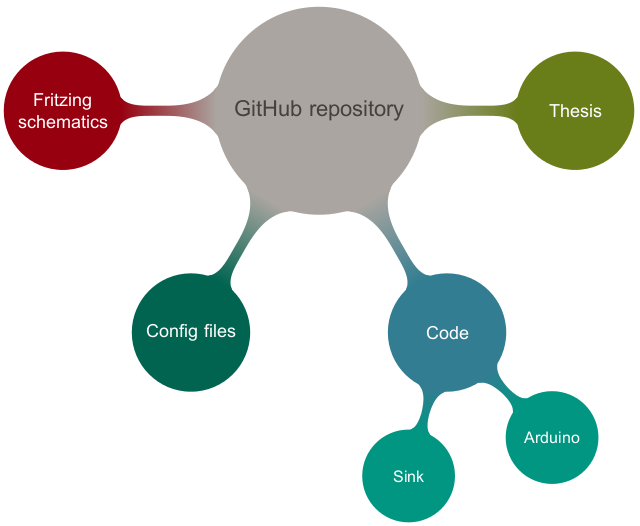
\includegraphics[width=\linewidth]{./Figures/github_repo.png}
        \rule{35em}{0.5pt}
        \caption[Structure of the GitHub repository]{Structure of the GitHub repository.}
    \label{fig:repo}
\end{figure}

Technologies, as described in Chapter \ref{Chapter3} are well-tested and mature solutions, thus inferring the project the following two main features:

\begin{itemize}
    \item Flexibility --- The system is prepared to transmit heterogeneous information. Each node is able to transmit different information and the sink will decode it anyway. This allows a community to gather what each individual wants, or to achieve better granularity where needed. That is, someone might be interested in measuring temperature every two blocks and humidity every four blocks.
    \item Velocity of deployment --- To deploy this network, just the RF modules must be properly configured, as well as some small code tweaking. In other words, just sensor nodes have to be adapted to particular needs, the sink will work anyway.
\end{itemize}


%----------------------------------------------------------------------------------------
%	SECTION 1
%----------------------------------------------------------------------------------------

\section{Network topology}

Network topology refers to the way nodes that conform the system are arranged, thus it is clear that this factor will determine very important components about the network, such as reliability, modularity, fault occurence, etc. The use of Digi Xbee\textregistered{} RF modules enables the network to be configured in any kind of topology, from a simple star to a complex mesh\footnote{Networks where a packet can follow more than one path to reach its destination.}. An example of such networks is depicted in figure \ref{fig:MeshNet}, where each circle represents a node and the lines the wireless links between them.

\begin{figure}[htbp]
    \centering
        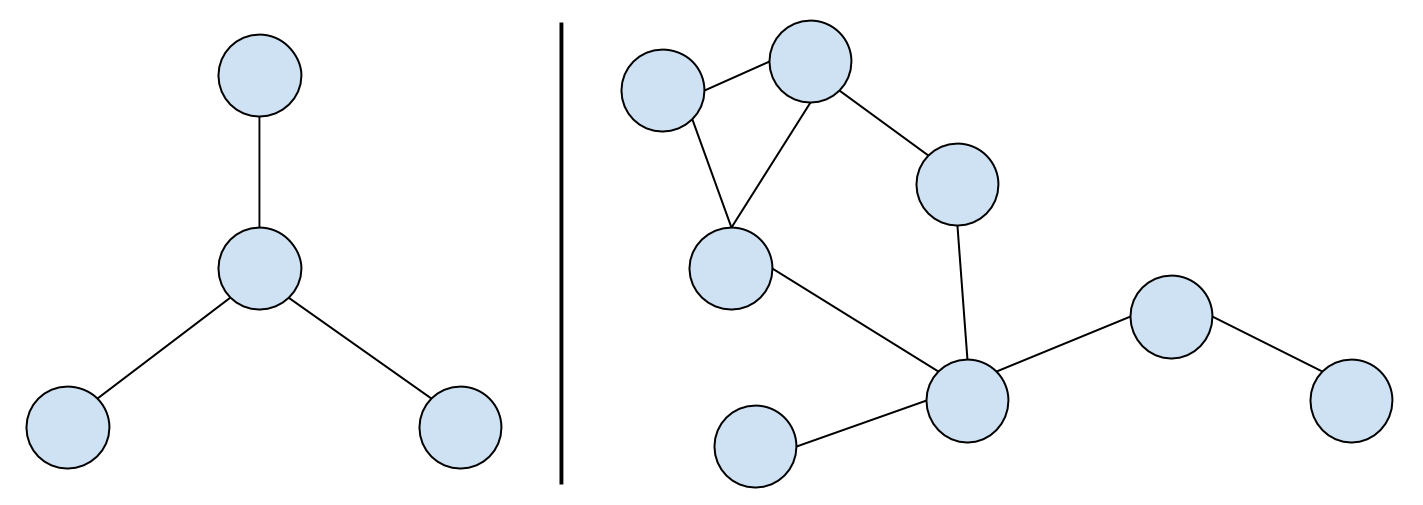
\includegraphics[scale=0.29]{./Figures/mesh_network.png}
        \rule{35em}{0.5pt}
        \caption[Mesh Network]{(Left) Star network topology; (Right) Mesh network topology.}
    \label{fig:MeshNet}
\end{figure}

As these RF devices only allow one single sink per network, not making use of mesh topologies would be an enormous drawback, since packet delivery would be subject to other nodes availability. Luckily, ZigBee specification allows enable some nodes to act as a relay for other nodes, enabling us to build complex networks with redundant paths. This statement, translated to battery-powered systems means that the more relay nodes a network has, the more prolonged the network's lifetime will be\cite{hou2005energy}, since relay nodes will have to pass on less messages. This is true except in the case the topology is a chain\footnote{In a chain topology (also called linear topology), each node has a two-way link with another node.}.


A mesh sensor network of this kind can be fully connected ---each node is connected to every other one--- or partially connected. This topology brings many advantages. They basically enable the system to be:

\begin{itemize}
    \item Self-healing --- Allows the network to operate when a node goes down.
    \item Self-routing --- When a packet is transmitted or forwarded, the route that it follows is created ---that is, calculated--- locally within every node.
    \item Self-forming --- Nodes that are new to the network create links automatically with the rest of nodes and routes are created dinamically as well.
\end{itemize}

The mentioned features and constraints imply that the first step to build such a network will begin by placing a sink and then start building from there, progressively reaching more distant places.

%-----------------------------------
%	SUBSECTION 1
%-----------------------------------
\subsection{Device roles}

Inside an ZigBee network there are three roles that a node can assume: coordinator, router and end device.

A \emph{coordinator} is the sink of the network, and as stated before, only one is allowed per network. A coordinator stores vital information about the network, acts as well as the trust center\footnote{Stores the keys if encryption is enabled, deciding who may or may not join the network.} and manages network security in general\cite{sensornetworktc}. In this case, it will be connected to the Raspberry Pi so data can be processed and uploaded to the Internet.

A \emph{router} can be understood as the previously mentioned relay nodes. It can generate and transmit data by itself to other router or to a coordinator but it is also able to forward packets from other nodes. If the network is very redundant it should not be a problem having a battery-powered router. If that is not the case, this option could lead to data outage, since packets from the edge of the network could not be forwarded.

Finally, an \emph{end device} is the least capable device of all. It can only transmit information that will be or will not be forwarded, thus they are always on the edge of the network. Since no other node depends on an end device, they can make use of the \emph{sleep mode}. This mode allows an XBee radio to wake up certain amout of time, transmit whatever it has to and then go back to sleep again. This mode is very energy efficient.

An example of such a network can be seen in figure \ref{fig:ZBeeNet}.

\begin{figure}[htbp]
    \centering
        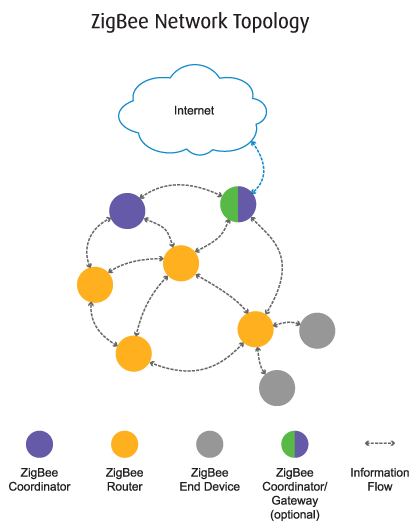
\includegraphics[scale=0.7]{./Figures/zigbee_topology.png}
        \rule{35em}{0.5pt}
        \caption[ZigBee network example]{An example of an ZigBee network, taken from the ZigBee Alliance website (\url{http://zigbee.org}).}
    \label{fig:ZBeeNet}
\end{figure}

%----------------------------------------------------------------------------------------
%	SECTION 2
%----------------------------------------------------------------------------------------

\section{Sensor nodes}

A sensor node is an element inside a wireless sensor network that is capable of gathering information, has some processing power and can relay information (if needed) to other nodes in the network\cite{chong2003sensor}.

In the design of this network two feasible scenarios have been considered, depending on which kind of sensors need to be used ---whether they are digital or analogic---, and if processing power is required. In case at least one of those features is needed, an Arduino plus an XBee\textregistered{} module are coupled together, with sensors attached to the board. Otherwise a standalone XBee\textregistered{} is used since it has a built-in ADC\footnote{An analog-to-digital converter takes a continous value --voltage, in our case-- as its input and converts it to a digital numeral.}, hence being able to directly read information from analog sensors.

These two operational modes have been taken in consideration because despite one of them can equate the other's characteristics one can think of some applications where the features of an additional microcontroller are just not needed. For instance, a sensor network monitoring temperature in an industrial environment just needs the so-mentioned analog-to-digital converter and a transceiver. Although there are two types of nodes, both can be used at the same time inside a given network.

To configure the radio of a sensor node one must use X-CTU, a piece of software developed by Digi International that, although it is intended to be run on Windows, it works fine on GNU/Linux using Wine\footnote{Wine is open source software that helps running Microsoft Windows applications on Unix-like operating systems.}, as it can be seen in figure \ref{fig:xctuonubuntu}.

\begin{figure}[htbp]
    \centering
        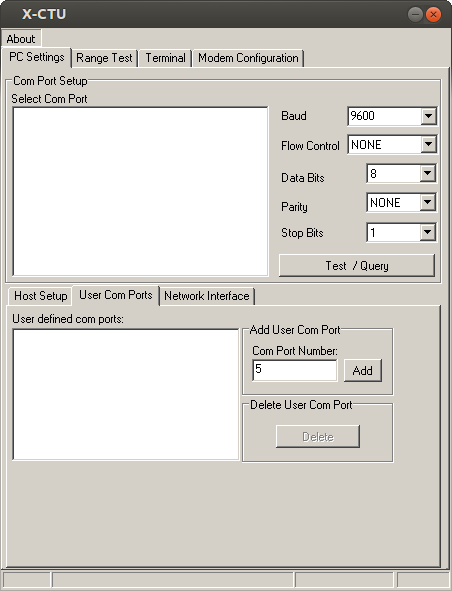
\includegraphics[scale=0.6]{./Figures/xctuonubuntu.png}
        \rule{35em}{0.5pt}
        \caption[Screenshot of X-CTU]{A screenshot of X-CTU running on Ubuntu 12.04 under Wine.}
    \label{fig:xctuonubuntu}
\end{figure}

In the next subsections it will be presented how these two types of sensor nodes are wired, how do they work and how are they configured.


%-----------------------------------
%	SUBSECTION 1
%-----------------------------------
\subsection{Standalone XBee}

To collect data directly from an XBee\textregistered{}, we need to make use of the analog-to-digital converters mentioned in section \ref{sec:xbee}. In figure \ref{fig:XBeeBO} we can observe the pinout of an XBee radio, with all its DIO (digital input output) pins. For analog input, we can only use from \texttt{DIO0} (sometimes called as well \texttt{AD0}) to \texttt{DIO3} (or \texttt{AD3})\cite{faludi2010building}.

\begin{figure}[htbp]
    \centering
        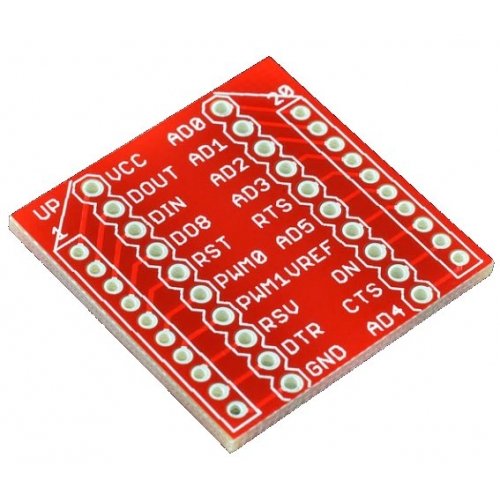
\includegraphics[scale=0.25]{./Figures/xbee_breakout.jpg}
        \rule{35em}{0.5pt}
    \caption[XBee pinout]{XBee pinout, seen from a breakout board.}
    \label{fig:XBeeBO}
\end{figure}

An schematic of this node can be seen below (figure \ref{fig:StandaloneXBee}), where only light level and temperature are measured. This particular setup could be useful for example to prevent fires in forests (although the optimal setup should have a humidity sensor as well).

\begin{figure}[htbp]
    \centering
        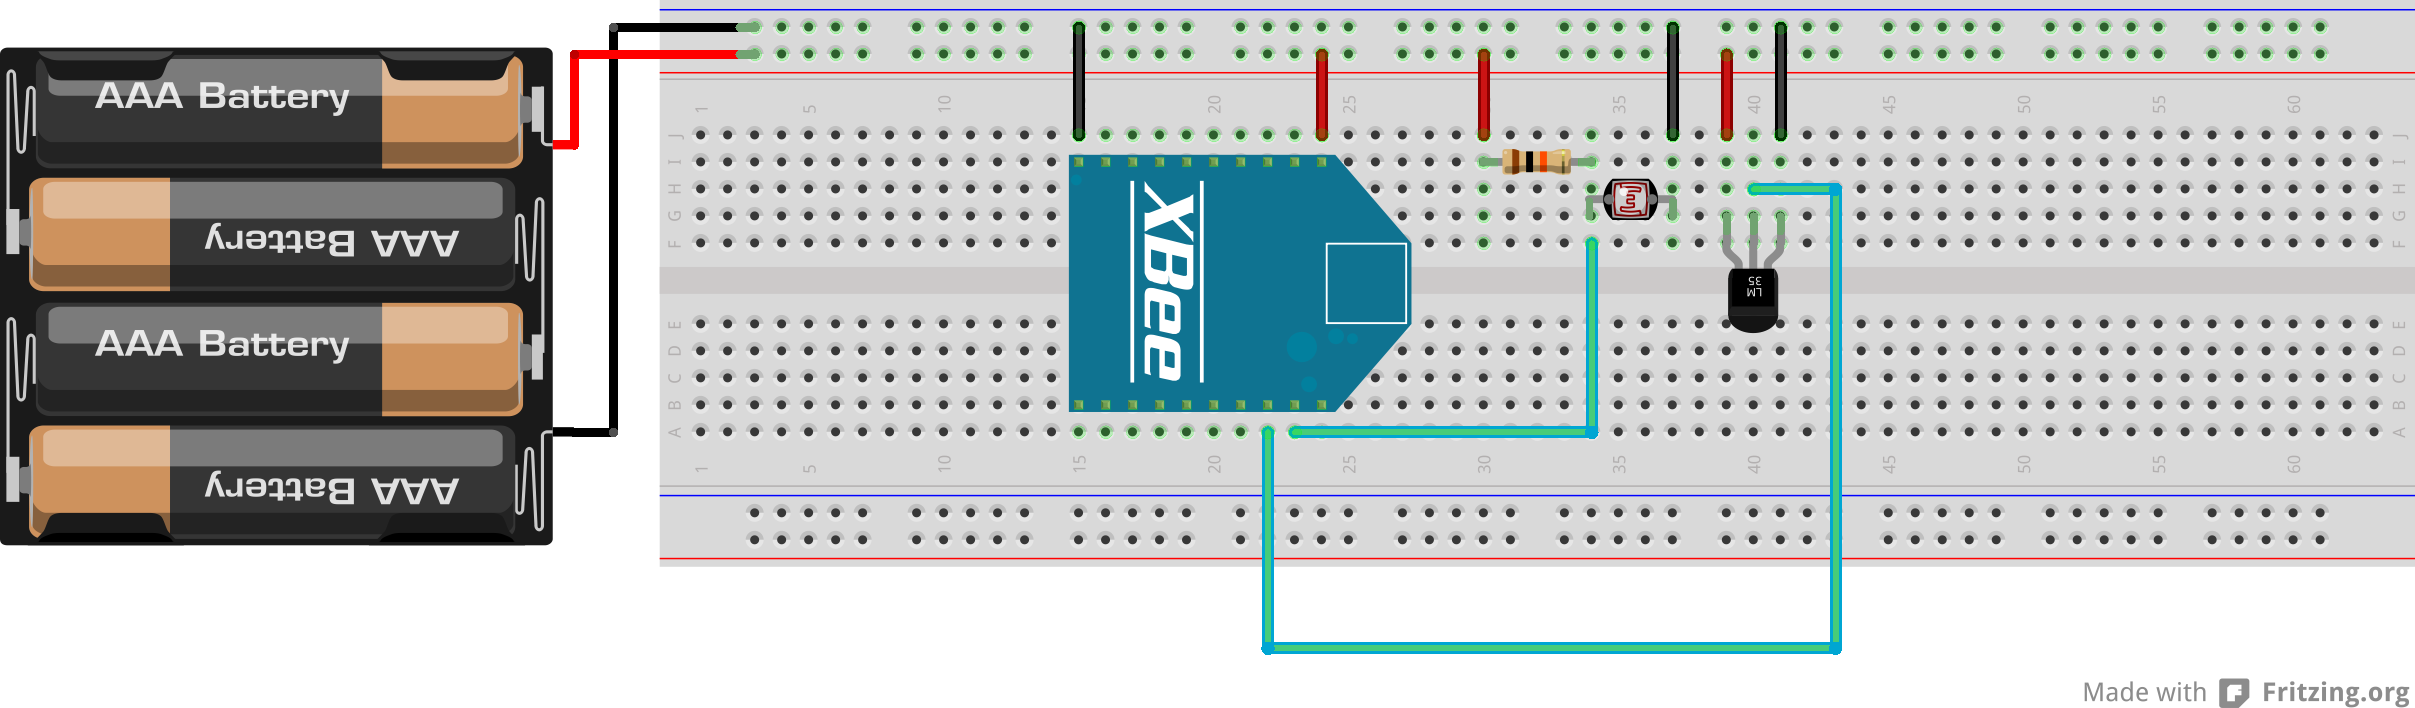
\includegraphics[scale=0.6]{./Figures/standalonexbee.png}
        \rule{35em}{0.5pt}
    \caption[Standalone XBee]{A standalone XBee node.}
    \label{fig:StandaloneXBee}
\end{figure}

Here, with the help of four AAA batteries we power an XBee\textregistered{} as well as the other sensors placed in the prototyping board. The temperature sensor (subsection \ref{sub:lm35}) has a dedicated output pin, which is directly attached to an analog input pin. As for light levels, the used LDR resistance\footnote{A photoresistor whose resistance varies depending on the surrounding light level.} does not have an output pin, and this is why we have to collect the sensory value through a voltage divider.

Using a battery and a solar panel to power a sensor node like this one, along with \emph{sleep mode} can result in very long lifetimes.

% ###############################
% # CONFIGURING STANDALONE XBEE #
% ###############################
\subsubsection{Configuring a standalone XBee\textregistered{}}
\label{subsub:coxbee}

The first step is to flash the radio module with the correct firmware, that is, with the \texttt{XB24-ZB} firmware. This \texttt{ZB} firmware implements the ZigBee 2007 specification\footnote{At the time of writing, the latest specification is from 2012.}. Also, a function set (or role) has to be set, as shown in figure \ref{fig:xctuw}.

\begin{figure}[htbp]
    \centering
        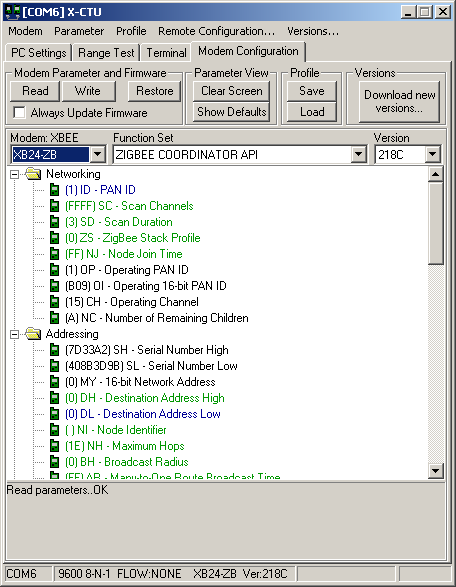
\includegraphics[scale=0.6]{./Figures/xctuw.png}
        \rule{35em}{0.5pt}
        \caption[XBee\textregistered{} configuration through X-CTU]{XBee\textregistered{} configuration through X-CTU.}
    \label{fig:xctuw}
\end{figure}

To configure a standalone node one must ensure that the RF module has the same \texttt{PANID} than the coordinator ---that is, the same network---. Also, API mode shall be enabled, thus setting the \texttt{AP} parameter to \texttt{2}, which means not only that API mode must be used but also \emph{escaping}. This \texttt{AP} parameter must be set to \texttt{2} because the Arduino based node only works with escaping enabled (as described in the next subsection). Thus, to achieve a certain degree of homogeneity both the nodes and the sink need to have this parameter explicitly enabled.

With escaping mode the system escapes some special characters. In other words, if special characters appear in the packet ---for instance \texttt{0x7E}, which serves as a start frame delimiter--- they are replaced by other sequences so they can be decoded as well by the receiver but without causing any trouble in the interpretation phase. Receiving an arbitrary \texttt{0x7E} could pose many problems for the receiver. It would not know when a packet really starts\cite{digi:escapedchars}.

Since we want to transmit samples periodically, we must configurate a sampling rate inside X-CTU, with the parameter \texttt{IR}. This value must be hexadecimal, so if for instance we want the module to transmit values every second, we must set \texttt{IR} to \texttt{3E8} ---or 1000ms---.

Finally, parameters \texttt{D0}, \texttt{D1}, \texttt{D2} and \texttt{D3} can be set to \texttt{2}, which will mean they are in ADC mode. In other words, for each sensor wired to one of these pins, one must configure those pins to work in the proper mode.

% TODO - Adjust repo
Example configuration files were exported from X-CTU and can be freely downloaded from the original git repository\footnote{\url{https://github.com/aandreuisabal/OSN}}. More precisely, they can be found in the \texttt{Config/X-CTU} folder.

%-----------------------------------
%	SUBSECTION 2
%-----------------------------------
\subsection{Arduino-based node}

Arduino is capable of executing C code, thus being able to process any kind of information no matter how complex it is (always bearing in mind its hardware limits). To transmit all the information, the RF module attached to it will be configured as described in subsection \ref{sub:xbeearduino}.

As a proof of concept, the example setup I have worked with has an analog sensor that measures sound levels (\ref{sub:sound}), another one that measures air quality in terms of fine particles in the air (\ref{sub:sharp}) and a digital sensor that reads humidity and temperature (\ref{sub:dht}). A possible setup with these elements is shown in figure \ref{fig:ArduinoNode}.

Here, the Arduino board can be powered by batteries or by a more stable power supply. It is the very same board that powers the sensors and the XBee\textregistered{}. Thereby, information is gathered and finally transmitted through the RF module (more information in section \ref{subsub:arduinosketch}).

% TODO - Conseguir modelo de Fritzing para SHARP GP2Y1010AU0F
\begin{figure}[htbp]
    \centering
        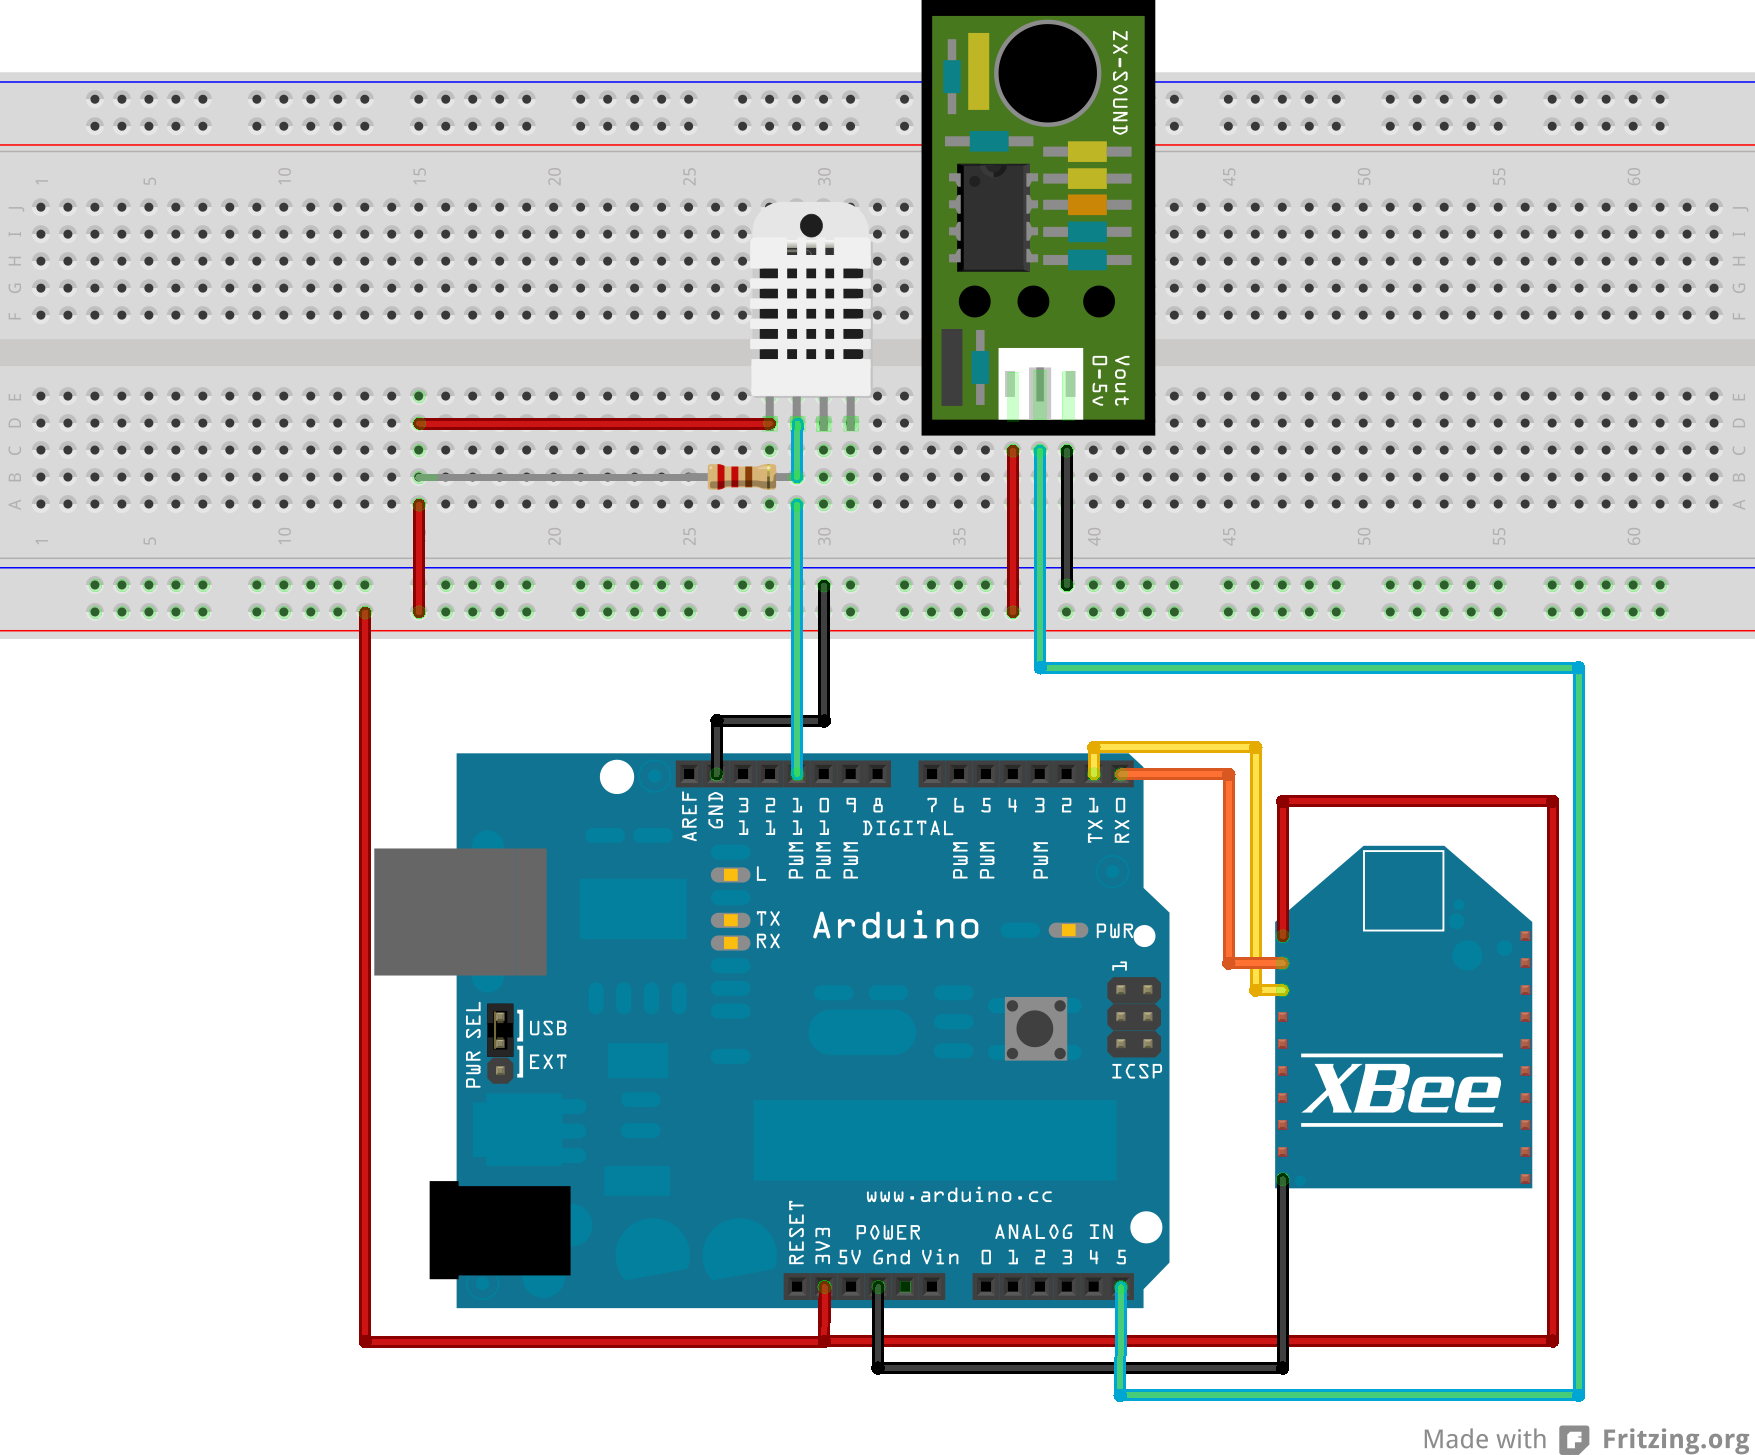
\includegraphics[scale=0.8]{./Figures/completesensornode.png}
        \rule{35em}{0.5pt}
    \caption[Arduino-based node schematic]{Sensor node based on Arduino.}
    \label{fig:ArduinoNode}
\end{figure}

This type of node has the same communication features as the standalone XBee. That is, encryption, acknowledgements, etc. Additionally, ACKs are better handled in this case since an Arduino can \emph{react} to them.

%-----------------------------------
%	SUBSUBSECTION 1
%-----------------------------------
\subsubsection{XBee\textregistered{} configuration}
\label{sub:xbeearduino}

The configuration for this type of node is quite simple. The same firmware and function set that were mentioned in subsection \ref{subsub:coxbee} have to be written in the XBee\textregistered{}.\texttt{PANID} must be set to the same than the coordinator's so they can interact with each other, and \texttt{AP} (that is, API mode) must be set to \texttt{2} to enable escaping.

%-----------------------------------
%	SUBSUBSECTION 2
%-----------------------------------
\subsubsection{Arduino sketch}
\label{subsub:arduinosketch}
A sketch is nothing more than the program an Arduino runs. The basic code is written in C/C++, and it consists of a main file ---with \texttt{.ino} extension--- and the XBee\textregistered{} libraries. The code can be browsed and downloaded via GitHub. There are two versions of the sketch:

\begin{itemize}
    \item Exact same code I used to conduct the experiments, so anyone can verify and/or test the obtained results.
    \item A skeleton file, that follows a very minimalistic approach in terms of lines of code but fully commented. This way, it can be extended as desired to build a sensor network from scratch with customized sensor nodes.
\end{itemize}

Arduino IDE is based on Processing IDE\footnote{\url{http://processing.org}}, and it follows the same structure than the Processing programming language. There are two main functions necessary for every program to work, namely \texttt{setup()} and another one called \texttt{loop()}. Respectively:

\begin{itemize}
    \item The \texttt{setup()} funcion initializes variables, modules (such as the XBee), libraries and sets pins in specific modes. After this function is successfully executed \texttt{loop()} is immediately called.
    \item \texttt{loop()} is a function that as its own name indicates, is executed over and over again. Thus inside this structure is where the action takes place. 
\end{itemize}

In our case, even before \texttt{setup()} starts, the following steps take place:

\begin{itemize}
    \item An object of type \texttt{XBee} is created, so serial information can be exchanged between the microcontroller and the RF module. 
    \item Additional information useful for the transmission is set: destination address (by default \texttt{0x0000000000000000}\footnote{This address is used to simply reach the coordinator. It is possible to write the specific address of the XBee ---which is written in the RF module--- as well.}), how big the packet will be, etc.
    \item Also, an array called \texttt{payload} is initialized, which will contain all readings as well as some \emph{metadata}. 
    \item The variables that will hold the different readings are also declared outside the two main function so they are recognized in a global scope.
    \item Finally, auxiliary C unions\footnote{An union allows us to represent information in more than one way. In our case it helps us convert integers, booleans, etc. into byte-level data.} are created. One for every compatible data type.
\end{itemize}

In our \texttt{setup()} step we initialize a serial connection with the XBee\textregistered{} and set a pin to act as digital output. This pin is the number \texttt{13}, which is connected to the on-board LED.

Then, in \texttt{loop()} all sensory values are recollected and then transmitted via a ZigBee packet. Finally, if the previously mentioned LED blinks once that will mean transmission took place successfully, otherwise it will blink twice. This last feature is especially interesting when debugging.

In figure \ref{fig:ArduinoProgram} it is depicted how the program works in more detail. This flowchart follows a top-down approach. That is, from general to more specific functions.

\begin{figure}[htbp]
    \centering
        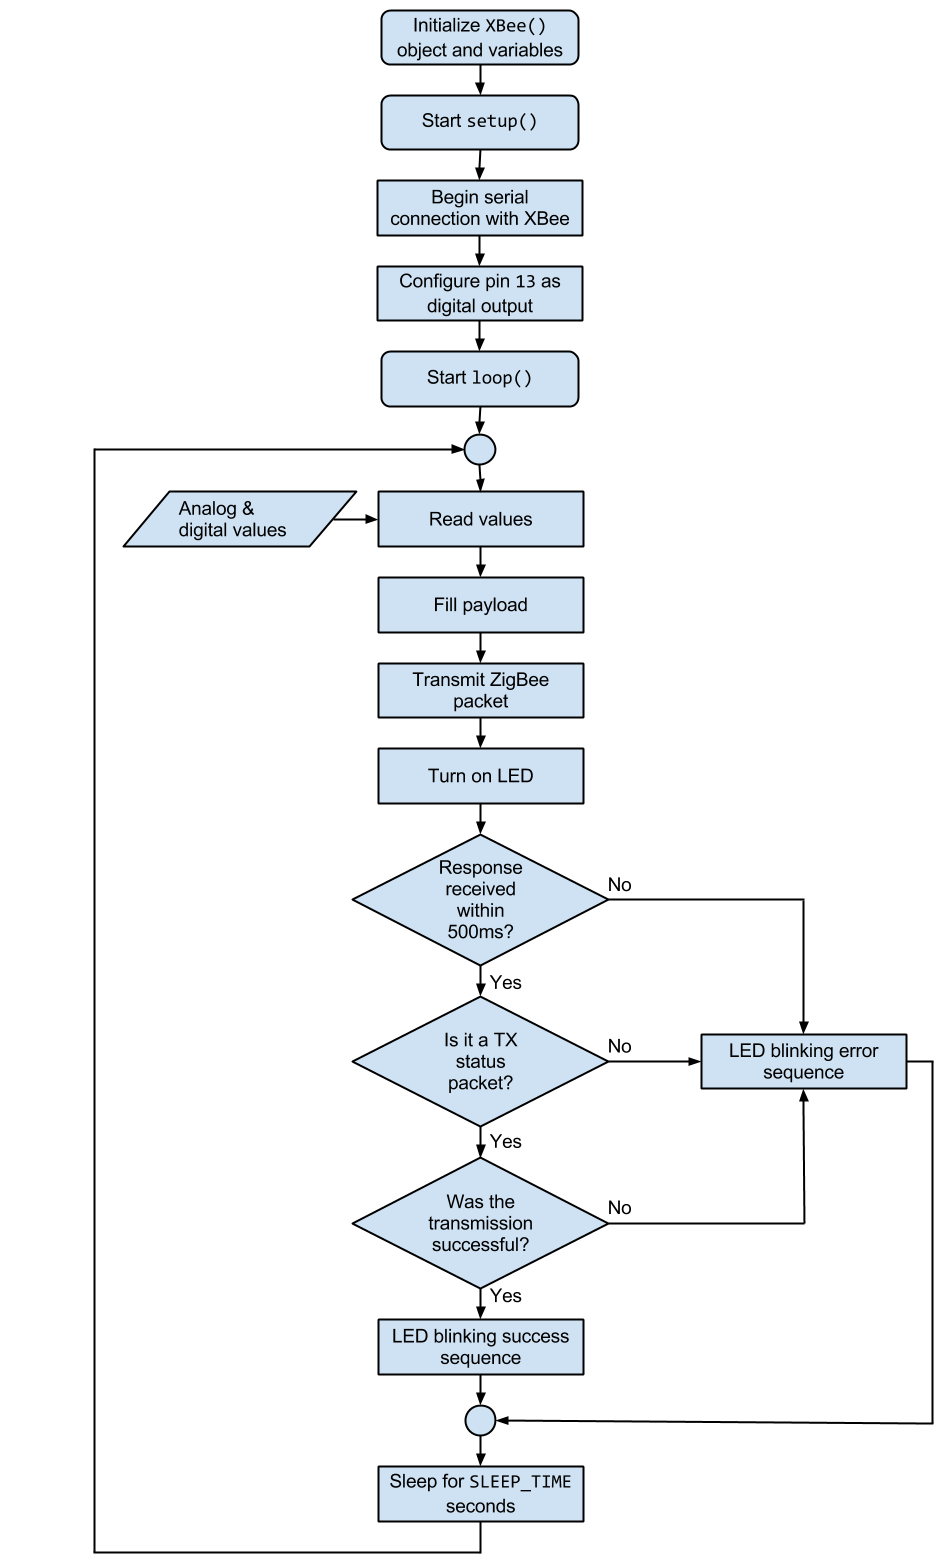
\includegraphics[scale=0.35]{./Figures/SensorNodeDia.png}
        \rule{35em}{0.5pt}
    \caption[Flow diagram of an Arduino-based node]{Flow diagram of the Arduino program.}
    \label{fig:ArduinoProgram}
\end{figure}

As for how values are read from the Arduino, figure \ref{fig:readvalues} explains how this process takes place step by step. Basically, digital values are read one time since the readings are more precise, and when reading an analog value the Arduino computes an average of \texttt{n} samples to smoothe the values from ``jumpy'' sensors.

\begin{figure}[htbp]
    \centering
        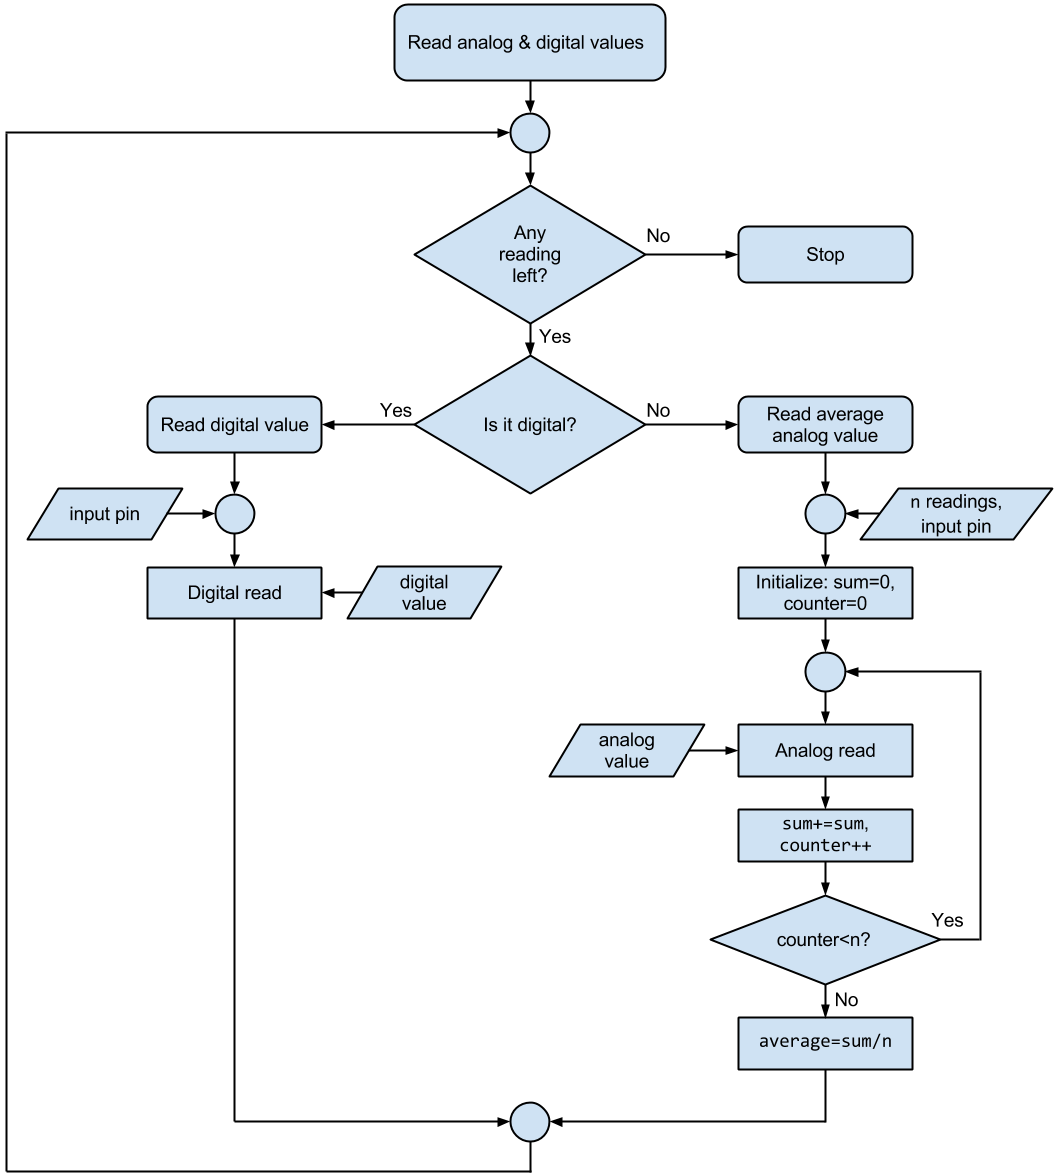
\includegraphics[scale=0.38]{./Figures/readvalues.png}
        \rule{35em}{0.5pt}
    \caption[Value reading flowchart]{Flowchart of how values are read.}
    \label{fig:readvalues}
\end{figure}

\paragraph{Working with metadata}
~\\
An initial requirement was that each sensor node can transmit whatever it needs to, I designed a rudimentary but efficient mechanism. At the start of every packet, an integer is sent. This is the only fixed value that every packet will hold. This integer will be tremendously helpful so the sink knows how to decode the payload ---keep in mind that data is sent in binary form---.

That is, the four first bytes of payload of every packet will be decoded as an unsigned integer at the sink --- which ranges from $0$ to ($2^{16}-1$)---. Then, each digit that conforms this number will be interpreted (one by one) as a unique data type, using table \ref{tab:mapnumbers}. The range of this unsigned integer is bigger when using other flavors of the Arduino, such as the Arduino Due\footnote{\url{http://arduino.cc/en/Guide/ArduinoDue}}.

\begin{table}[ht] 
\centering
\begin{tabular}{c|l}
Number          & Data type             \\
\hline
1               & \texttt{boolean}      \\
2               & \texttt{char}         \\
3               & \texttt{unsigned char}\\
4               & \texttt{int}          \\
5               & \texttt{unsined int}  \\
6               & \texttt{long}         \\
7               & \texttt{unsigned long}\\
8               & \texttt{short}        \\
9               & \texttt{float}        \\
0               & \texttt{double}       \\
\end{tabular}
\caption{Mapping between numbers and data types.}
\label{tab:mapnumbers}
\end{table}

To come up with an actual way to translate between digits and data types, I had a look at which data types the Arduino IDE could handle, and which of them Python can decode ---that is, which data types do they share---. For more information on supported data types one can visit the reference on the official Arduino webpage\footnote{\url{http://arduino.cc/en/Reference/HomePage}} and Python documentation on data structures\footnote{\url{http://docs.python.org/2/library/struct.html}}.

To give an example, let's say a node wants to transmit two floats and a boolean. According to table \ref{tab:mapnumbers}, this would yield the numbers \texttt{9}, \texttt{9} and \texttt{1}. Hence this number (\texttt{METADATA} in the code) can be any permutation using the following digits: \texttt{199}.

Nonetheless, it is recommended to first transmit the lowest values (starting with \texttt{1},\texttt{2}\ldots) and finishing with the highest ones (\ldots\texttt{9},\texttt{0}). This is because since the range of an \texttt{unsigned int} is somewhat small ---at least in a 8-bit architecture--- transmitting information in this order reduces the probabilities or exceeding that range (again, from $0$ to ($2^{16}-1$)).

In the current state of the code, this ``magic'' number has to be hardcoded. Once this number has been written in the \texttt{METADATA} variable, the information shall be sent in the same order. Following the previous example, this number would be \texttt{199}, thereby sending the boolean first and then the two remaining floats.

\paragraph{Packing information}
~\\
Information is packed with the help of unions, as stated before. A union is declared as follows:

\begin{verbatim}
union u_boolean {
    uint8_t b[1];
    boolean boolean;
} boolean_union;
\end{verbatim}

This means that the union named \texttt{boolean\_union} will translate indifferently between a boolean and a byte. Later on, the \texttt{payload} variable ---which as its own name indicates, holds the payload--- shall be filled with the data (including the metadata):

\begin{verbatim}
boolean_union.boolean = sample_boolean;
for (int i=0;i<BOOLEAN_SIZE;i++){
    payload[i]=boolean_union.b[i];
}
\end{verbatim}

Although these lines of code seem ``messy'' at first glance its functionality is quite simple. It just loads the payload with byte information.


%----------------------------------------------------------------------------------------
%	SECTION 3
%----------------------------------------------------------------------------------------

\section{Network sink}

The sink is where all the information is headed. As stated in the previous section, it is composed of a Raspberry Pi with an XBee module connected to it. The schematic, although simple can be seen in the figure \ref{fig:sinkrpi}. Note that in the figure there is not an XBee but a breakout board for it that has a miniUSB interface, very useful for our purposes. On top of it there is the actual XBee\textregistered{}.

\begin{figure}[htbp]
    \centering
        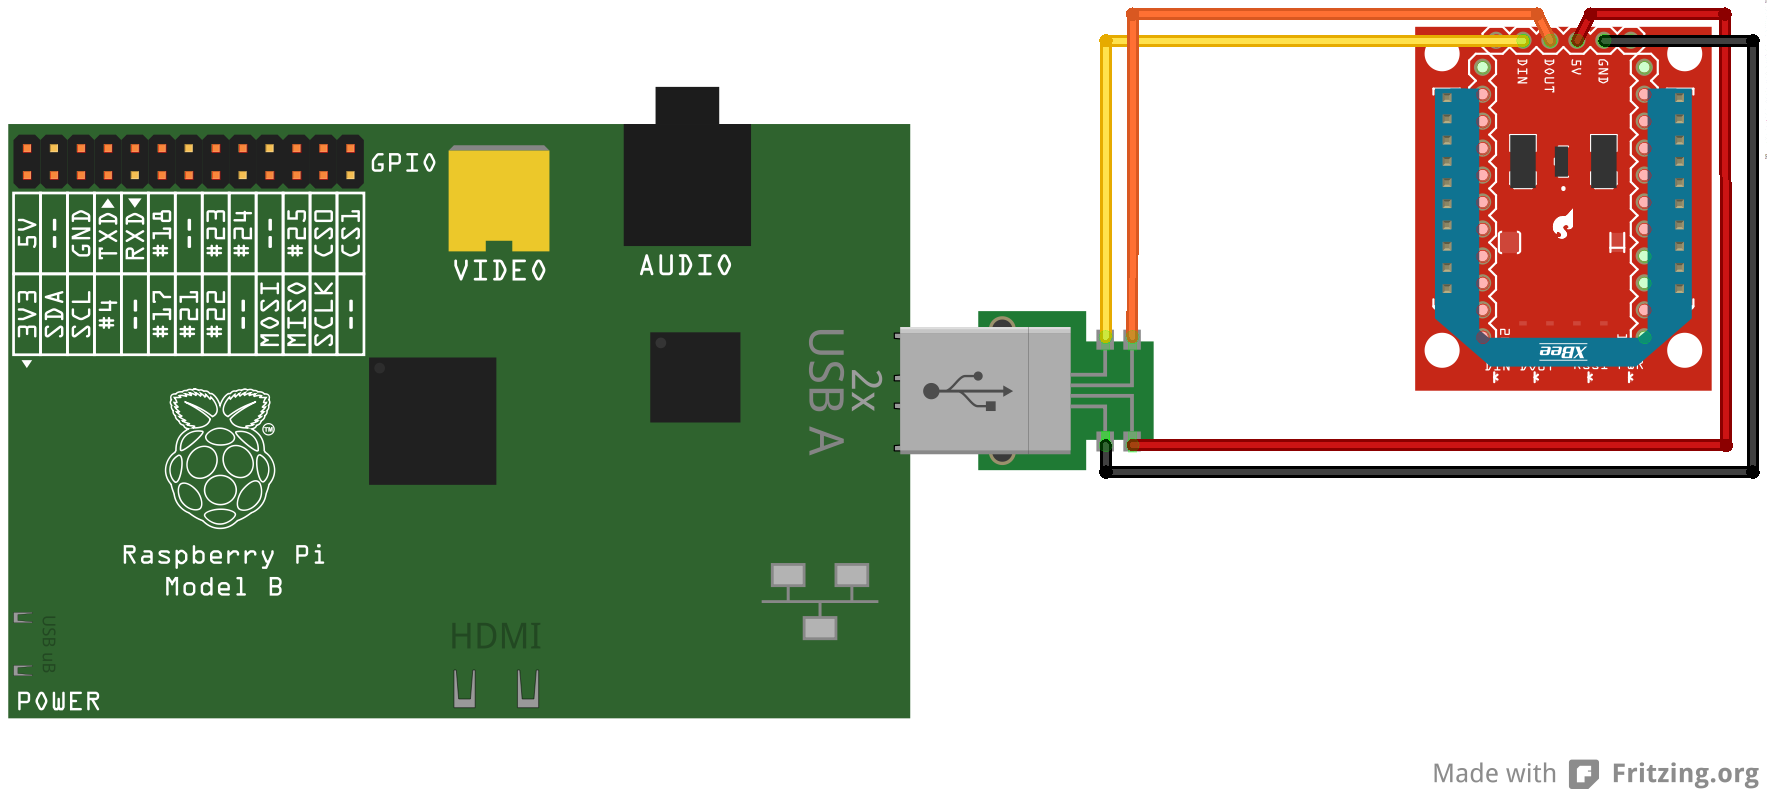
\includegraphics[scale=0.7]{./Figures/server_side.png}
        \rule{35em}{0.5pt}
    \caption[Raspberry Pi based sink]{Schematic of the sink.}
    \label{fig:sinkrpi}
\end{figure}

The GNU/Linux distribution that has been chosen to operate in this device is Arch Linux ARM, as stated in section \ref{sec:alarmmm}. Its repositories are huge because regular users contribute to a non-official repository, called ``Arch User Repository'' (also known as AUR). There, all the packages mentioned in chapter \ref{Chapter3} are available without compiling from source ---in the form of binaries---.

The script, called \texttt{server.py} is then run as a daemon which will be always receiving information. It needs two arguments:

\begin{itemize}
    \item Device file that interfaces with the XBee\textregistered{} (e.g. \texttt{/dev/ttyUSB0}). Depending on the devices already attached to the computer the last number might change.
    \item Baud rate the XBee\textregistered{} is working at (e.g. \texttt{9600}). Can be customized via X-CTU.
\end{itemize}

What the script basically does is run an asynchronous \texttt{XBee} dispatcher, which will create a new background thread for every new packet that arrives, thus enabling the sink to process many packets at the same time without blocking the whole script. The program is quite modular, since it allows to upload the information to the website the user wants by just uncommenting certain lines. A more detailed view on how it generally works can be seen in figure \ref{fig:sindia}.

\begin{figure}[htbp]
    \centering
        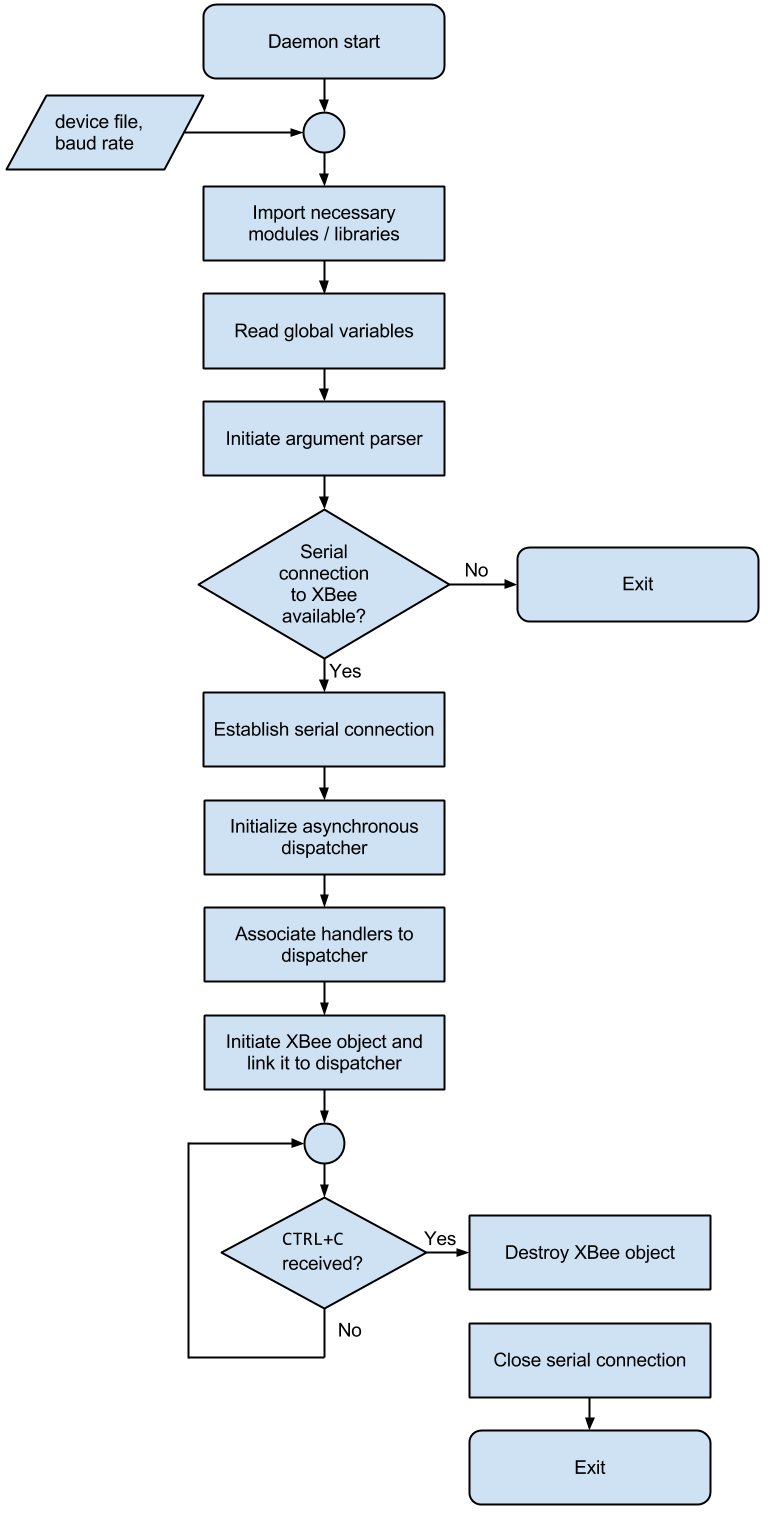
\includegraphics[scale=0.35]{./Figures/sindia.png}
        \rule{35em}{0.5pt}
    \caption[Flow diagram of the sink script]{Flow diagram of the sink script.}
    \label{fig:sindia}
\end{figure}

However, in figure \ref{fig:sindia} we cannot appreciate how packets are actually handled, and what happens to them afterwards. For that matter, figures \ref{fig:phandler} and \ref{fig:puploader} explain these two phases more precisely.

\begin{figure}[htbp]
    \centering
        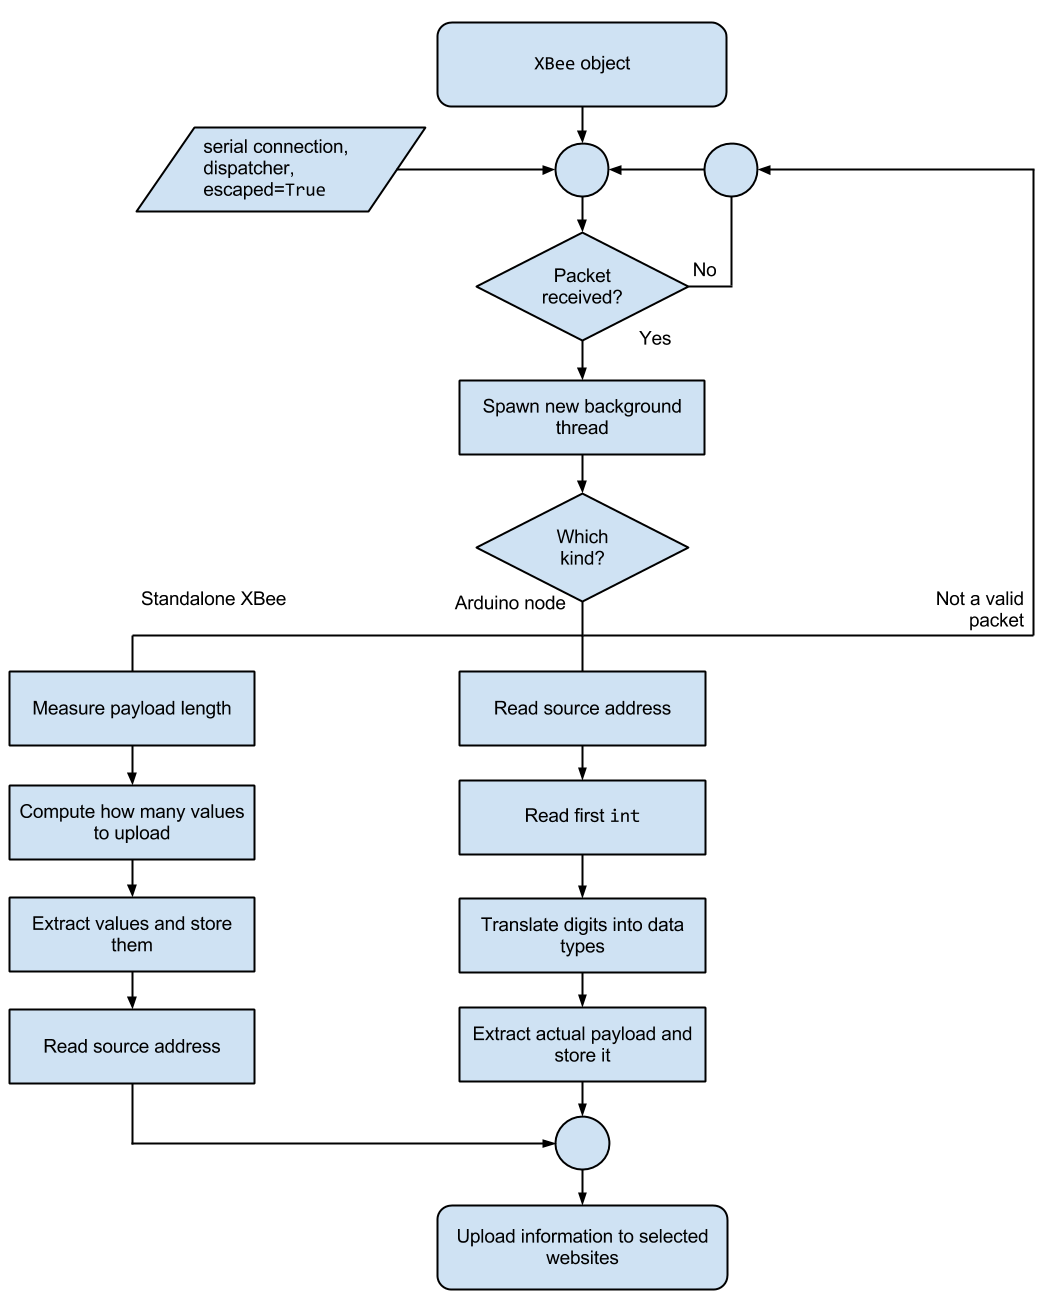
\includegraphics[scale=0.38]{./Figures/packet_handler.png}
        \rule{35em}{0.5pt}
    \caption[Packet dispatcher flowchart]{Flowchart of how packets are dispatched.}
    \label{fig:phandler}
\end{figure}

\begin{figure}[htbp]
    \centering
        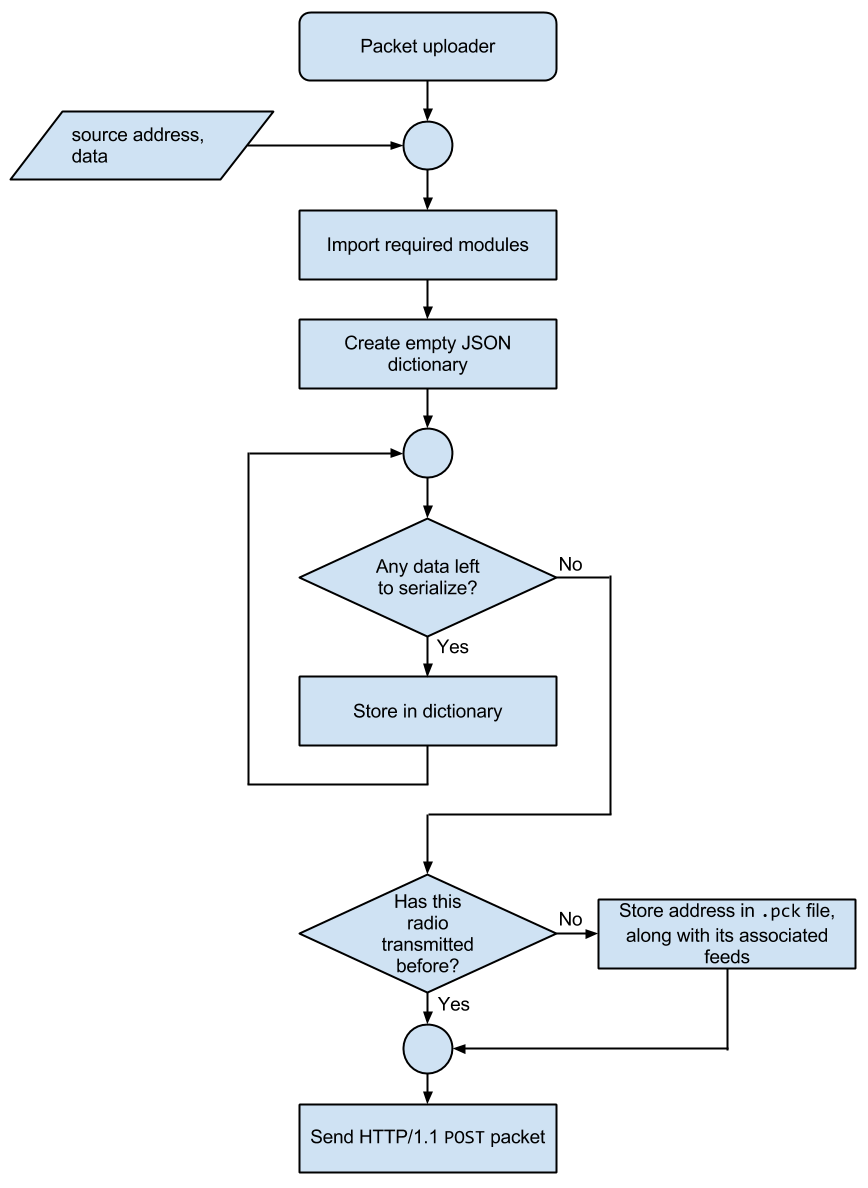
\includegraphics[scale=0.38]{./Figures/packet_uploader.png}
        \rule{35em}{0.5pt}
    \caption[Packet uploader flowchart]{How a packet uploader works.}
    \label{fig:puploader}
\end{figure}

At the moment of writing, two uploaders have been created. One for Xively\footnote{\url{http://xively.com}} and one for any Nimbits cloud\footnote{\url{http://nimbits.com}}. The results can be seen in chapter \ref{Chapter6}.

\subsection{Setting up the sink}

The XBee\textregistered{} settings that have to be set are the same that those on an Arduino node. That is, a certain \texttt{PANID} and the \texttt{AP} parameter set to \texttt{2}.

These are the steps related to the Raspberry Pi that have to be followed to get a functioning sink:

\begin{enumerate}
    \item Get a compatible SD card\footnote{\url{http://elinux.org/RPi_SD_cards}}, download the latest ISO image from the Arch Linux ARM website\footnote{\url{http://archlinuxarm.org/platforms/armv6/raspberry-pi}} and transfer it to the card. Depending on what operative system you are using you will want to use one tool or another (\texttt{dd} tool for *NIX-based operating systems, Win32DiskImager for Windows). If the operating system is correctly loaded in the SD card the Raspberry Pi shall boot properly and its LEDs will start blinking.
    \item To actually interact with the device, there are two options:
        \begin{itemize}
            \item Through a display that accepts HDMI input and a USB keyboard.
            \item Arch Linux ARM has the SSH\footnote{Secure Shell allows to remotely access another machine and remotely execute commands.} daemon enabled by default.
        \end{itemize}
    \item Arch Linux makes use of \texttt{pacman}, a wonderful package manager. From a terminal, issue the following command (requires root access): 
        \begin{verbatim}
            pacman -Syu \
            python2 python2-requests \
            python2-pyserial
        \end{verbatim}
    This will upgrade all the operating system packages and will install as well the necessary ones for the script to work.
    \item Clone the GitHub repository by issuing: 
        \begin{verbatim}
            git clone \
            git@github.com:aandreuisabal/OSN.git
        \end{verbatim} 
        This will clone the GitHub repository inside a folder called \texttt{OSN} in the current directory. There, inside \texttt{Code/server} folder there are all the necessary files to run the sink daemon.
    \item Modify the file \texttt{osn.service} so the path to the script is correctly set. Finally, move this file to \texttt{/etc/systemd/system/} and issue this command to start the script at boot time (requires root privileges):
        \begin{verbatim}
            systemctl enable osn
        \end{verbatim}
\end{enumerate}



%----------------------------------------------------------------------------------------
%	SECTION 4
%----------------------------------------------------------------------------------------
\section{Deploying the network}

To deploy this network one must first configure the coordinator as explained before, and start placing sensor nodes ---configured properly--- around until reaching the desired coverage. As for the script, one must first fill the necessary constants, such as API keys ---necessary to upload information to data clouds---, usernames and passwords. This last step is done through the modification of the uploader files (located in \texttt{Code/server/uploaders/*.py}), where variables denoted by capital letters hold this information. Each file refers to a data cloud where data shall be uploaded. So for instance, if you are willing to upload data to Xively, the user shall modify the file \texttt{uploaders/xively.py}.
